%%%%%%%%%%%%%%%%%%%%%%%%%%%%%%%%%%%%%%%%%
% University Assignment Title Page 
% LaTeX Template
% Version 1.0 (27/12/12)
%
% This template has been downloaded from:
% http://www.LaTeXTemplates.com
%
% Original author:
% WikiBooks (http://en.wikibooks.org/wiki/LaTeX/Title_Creation)
%
% License:
% CC BY-NC-SA 3.0 (http://creativecommons.org/licenses/by-nc-sa/3.0/)
% 
% Instructions for using this template:
% This title page is capable of being compiled as is. This is not useful for 
% including it in another document. To do this, you have two options: 
%
% 1) Copy/paste everything between \begin{document} and \end{document} 
% starting at \begin{titlepage} and paste this into another LaTeX file where you 
% want your title page.
% OR
% 2) Remove everything outside the \begin{titlepage} and \end{titlepage} and 
% move this file to the same directory as the LaTeX file you wish to add it to. 
% Then add \documentclass[12pt]{article}
\usepackage[english]{babel}
\usepackage{amsmath}
\usepackage{graphicx}
\usepackage{textcomp}
\usepackage{parskip}
\usepackage[colorinlistoftodos]{todonotes}
\usepackage{csquotes}
\usepackage{float}
\usepackage[backend=biber,style=ieee]{biblatex}
\addbibresource{bibliography.bib}

\begin{document}

\begin{titlepage}

\newcommand{\HRule}{\rule{\linewidth}{0.5mm}}
\center 

\textsc{\LARGE Iowa State University }\\[1.5cm] 
\textsc{\Large Center for Statistics and Applications in Forensic
Evidence
}\\[0.5cm] 

\HRule \\[0.4cm]
{ \huge \bfseries Shoe Print Data Collection: Additional Methods }\\[0.4cm] 
\HRule \\[1.5cm]



\begin{center}
\centering
 
\includegraphics[scale=.4]{csafe-logo}\\[1cm]
\end{center}







\end{titlepage}

\section{Introduction}

 When developing the methodology for the longitudinal shoe study conducted by the Center for Statistics and Applications in Forensic Evidence (CSAFE), collection procedures were designed to obtain the most ideal shoe-sole impression possible. While these images will be useful to the researcher and practitioner communities, they do not provide realistic examples of prints that would be collected from a crime scene/suspected crime scene. For this reason, CSAFE researchers have compiled this manual which contains procedures for further data collection and offers new, or edited, procedures that better represent the practices of current forensic examiners and crime scene teams. If at any time there is a question on any of these procedures, please make a note using a post-it note and e-mail the principal investigator, the project manager, the faculty in charge of the study, or the author of the specific procedure. 

\end{document} to your LaTeX file where you want your
% title page.
%
%%%%%%%%%%%%%%%%%%%%%%%%%%%%%%%%%%%%%%%%%
%\title{Title page with logo}
%----------------------------------------------------------------------------------------
%	PACKAGES AND OTHER DOCUMENT CONFIGURATIONS
%----------------------------------------------------------------------------------------

\documentclass[12pt]{article}
\usepackage[english]{babel}
\usepackage[utf8x]{inputenc}
\usepackage{amsmath}
\usepackage{graphicx}
\usepackage[colorinlistoftodos]{todonotes}

\begin{document}
\begin{titlepage}

\newcommand{\HRule}{\rule{\linewidth}{0.5mm}} % Defines a new command for the horizontal lines, change thickness here

\center % Center everything on the page
 
%----------------------------------------------------------------------------------------
%	HEADING SECTIONS
%----------------------------------------------------------------------------------------

\textsc{\LARGE Iowa State University}\\[1.75cm] % Iowa State University 
\textsc{\Large Center for Statistics and Applications in Forensic Evidence }\\[.5cm] % CSAFE
\textsc{\large CSAFE}\\[0.5cm] % Center for Statistics and Applications in Forensic Evidence 

%----------------------------------------------------------------------------------------
%	2D Shoe Scanner Procedure
%----------------------------------------------------------------------------------------

\HRule \\[0.4cm]
{ \huge \bfseries Data Collection: Longitudinal Shoe Study  }\\[0.4cm] % Title of your document
{ \Large \textit General Procedure and Subsequent Changes  }\\[0.2cm] % Title of your document
\HRule \\[1.5cm]
 
%----------------------------------------------------------------------------------------
%	AUTHOR SECTION
%----------------------------------------------------------------------------------------

\begin{minipage}{0.4\textwidth}
\begin{flushleft} \large
\emph{Author:}\\
  James \textsc{E. Kruse} % James E. Kruse
\end{flushleft}
\end{minipage}
~
\begin{minipage}{0.4\textwidth}
\begin{flushright} \large
\emph{Supervisor:} \\
Dr. Guillermo \textsc{Basulto-Elias} % Supervisor's Name
\end{flushright}
\end{minipage}\\[2cm]

% If you don't want a supervisor, uncomment the two lines below and remove the section above
%\Large \emph{Author:}\\
%John \textsc{Smith}\\[3cm] % Your name

%----------------------------------------------------------------------------------------
%	LOGO SECTION
%----------------------------------------------------------------------------------------

\includegraphics[scale=.5]{Logo}\\[1cm]

\begin{center}
\begin{tabular}{ c   |   c } 
 
\end{tabular}
\end{center}
%----------------------------------------------------------------------------------------
%	DATE SECTION
%----------------------------------------------------------------------------------------

{\large \today}\\[2cm] % Date, change the \today to a set date if you want to be precise


%----------------------------------------------------------------------------------------

\vfill % Fill the rest of the page with whitespace

\end{titlepage}

\tableofcontents

\newpage


%\bfseries 

\section{Introduction}

Before the baseline collection for this study began, a manual was developed.This manual laid out the procedure for each of the seven methods used during the longitudinal shoe study. Over the course of nine months, various experts, CSAFE researchers, faculty, and staff provided feedback on the images, prints, models and impressions with the end goal of creating the most realistic and workable data base possible. 

The purpose of this document is to map out these above mentioned changes to the collection methods. It is meant to be used in conjunction with the procedures manual and is not meant to be used as a step for step method for future data collection.  

The general procedure for each collection method will be described in full during the baseline portion of this document. Subsequent sections will then describe how the procedure changed, if any change occurred, and approximately when this change went into effect. 

\newpage

%\bfseries 
\subsection{Baseline}
After baseline collection had began and some shoes had been distributed, it was decided that a second replicate would be taken on select methods. Due to this, not all of the before mentioned shoes have replicates present in the baseline data set. 
   For shoes 6, 10, 24, 28, 29, 31, 37, 44, 53, 59, 61, 63, 64, 66, 84, 92, 103, 104, 115, 120, 122, 124, 138, 141, and 150 a second sample was taken during the film procedure and the 3D scanning procedure. 


\subsubsection{HR Pressure Mat}

 When participants arrived to collect their shoes at the beginning of the study, they were asked to step onto a pressure mat scanner. This scanner (Figure 1) is a product of Tekscan and allows us to collect a sample of both the way each participant steps and the points of the foot where the most pressure is placed. In some cases, this data was taken after the shoes had been worn due to inability to set up an initial meeting. 
   
   The area in which the scanner was located had spike tape marking the exact location of the device and a path leading both toward and away from it. This was to limit the variability in approach and to make communicating directions to the participants easier. 
   
   Participants themselves walked six times across the mat, per foot. Half of these were wearing nothing but a thin disposable sock (Figure 2) on the foot and the other half were wearing their shoe (Figure 3), or a new shoe of the same type. On the occasion that this procedure was done after the shoes had been worn, participants used their assigned shoes only. 
   
   Each scan was then saved as a video, two different CSV files, and as a jpg image. 
   
   It should be noted that this procedure was only preformed once for each pair of shoes. This was also the only procedure that involved the participant during the data collection process. 

\begin{figure}[!htp]
\centering
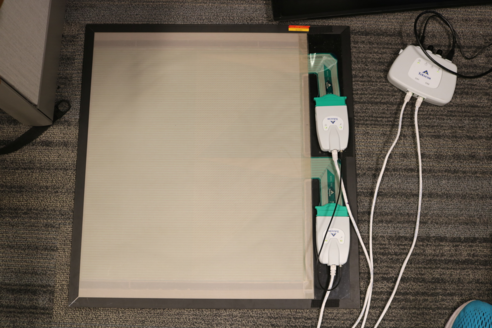
\includegraphics[width=8cm]{Mat_Scanner}
\caption{Mat Pressure Scanner by Tekscan }
\label{Image 1}
\end{figure}


\begin{figure}[!htp]
\centering
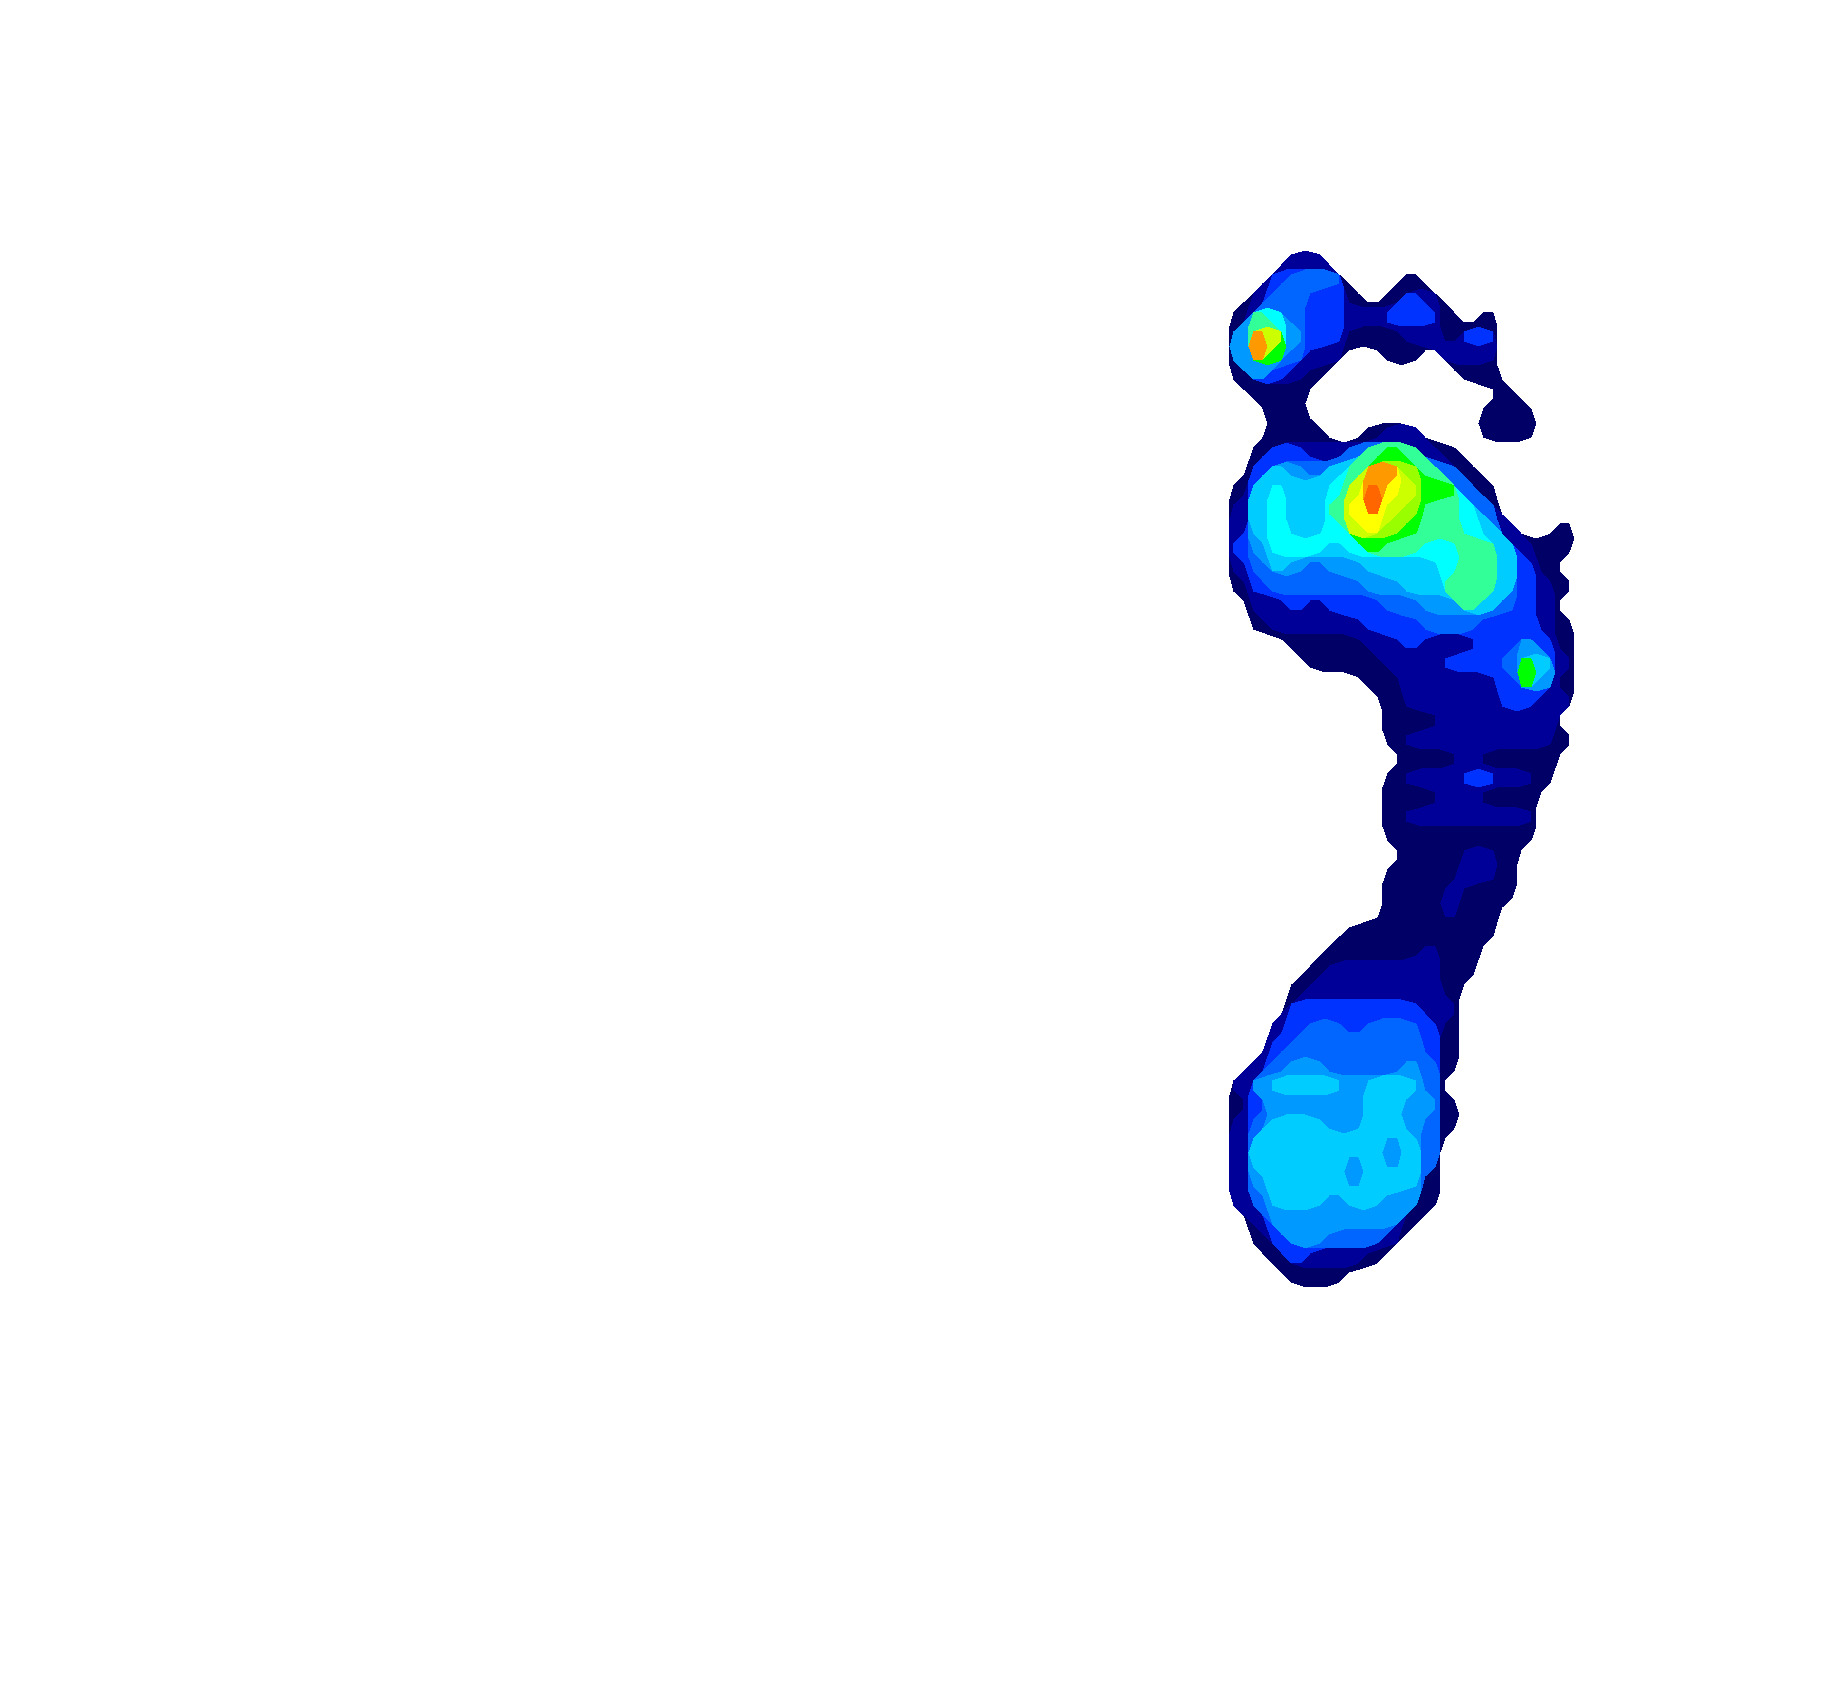
\includegraphics[width=8cm]{Mat_Foot}
\caption{Pressure map of a participants foot taken on the Mat Pressure Scanner}
\label{Image 2}
\end{figure}

\begin{figure}[!htp]
\centering
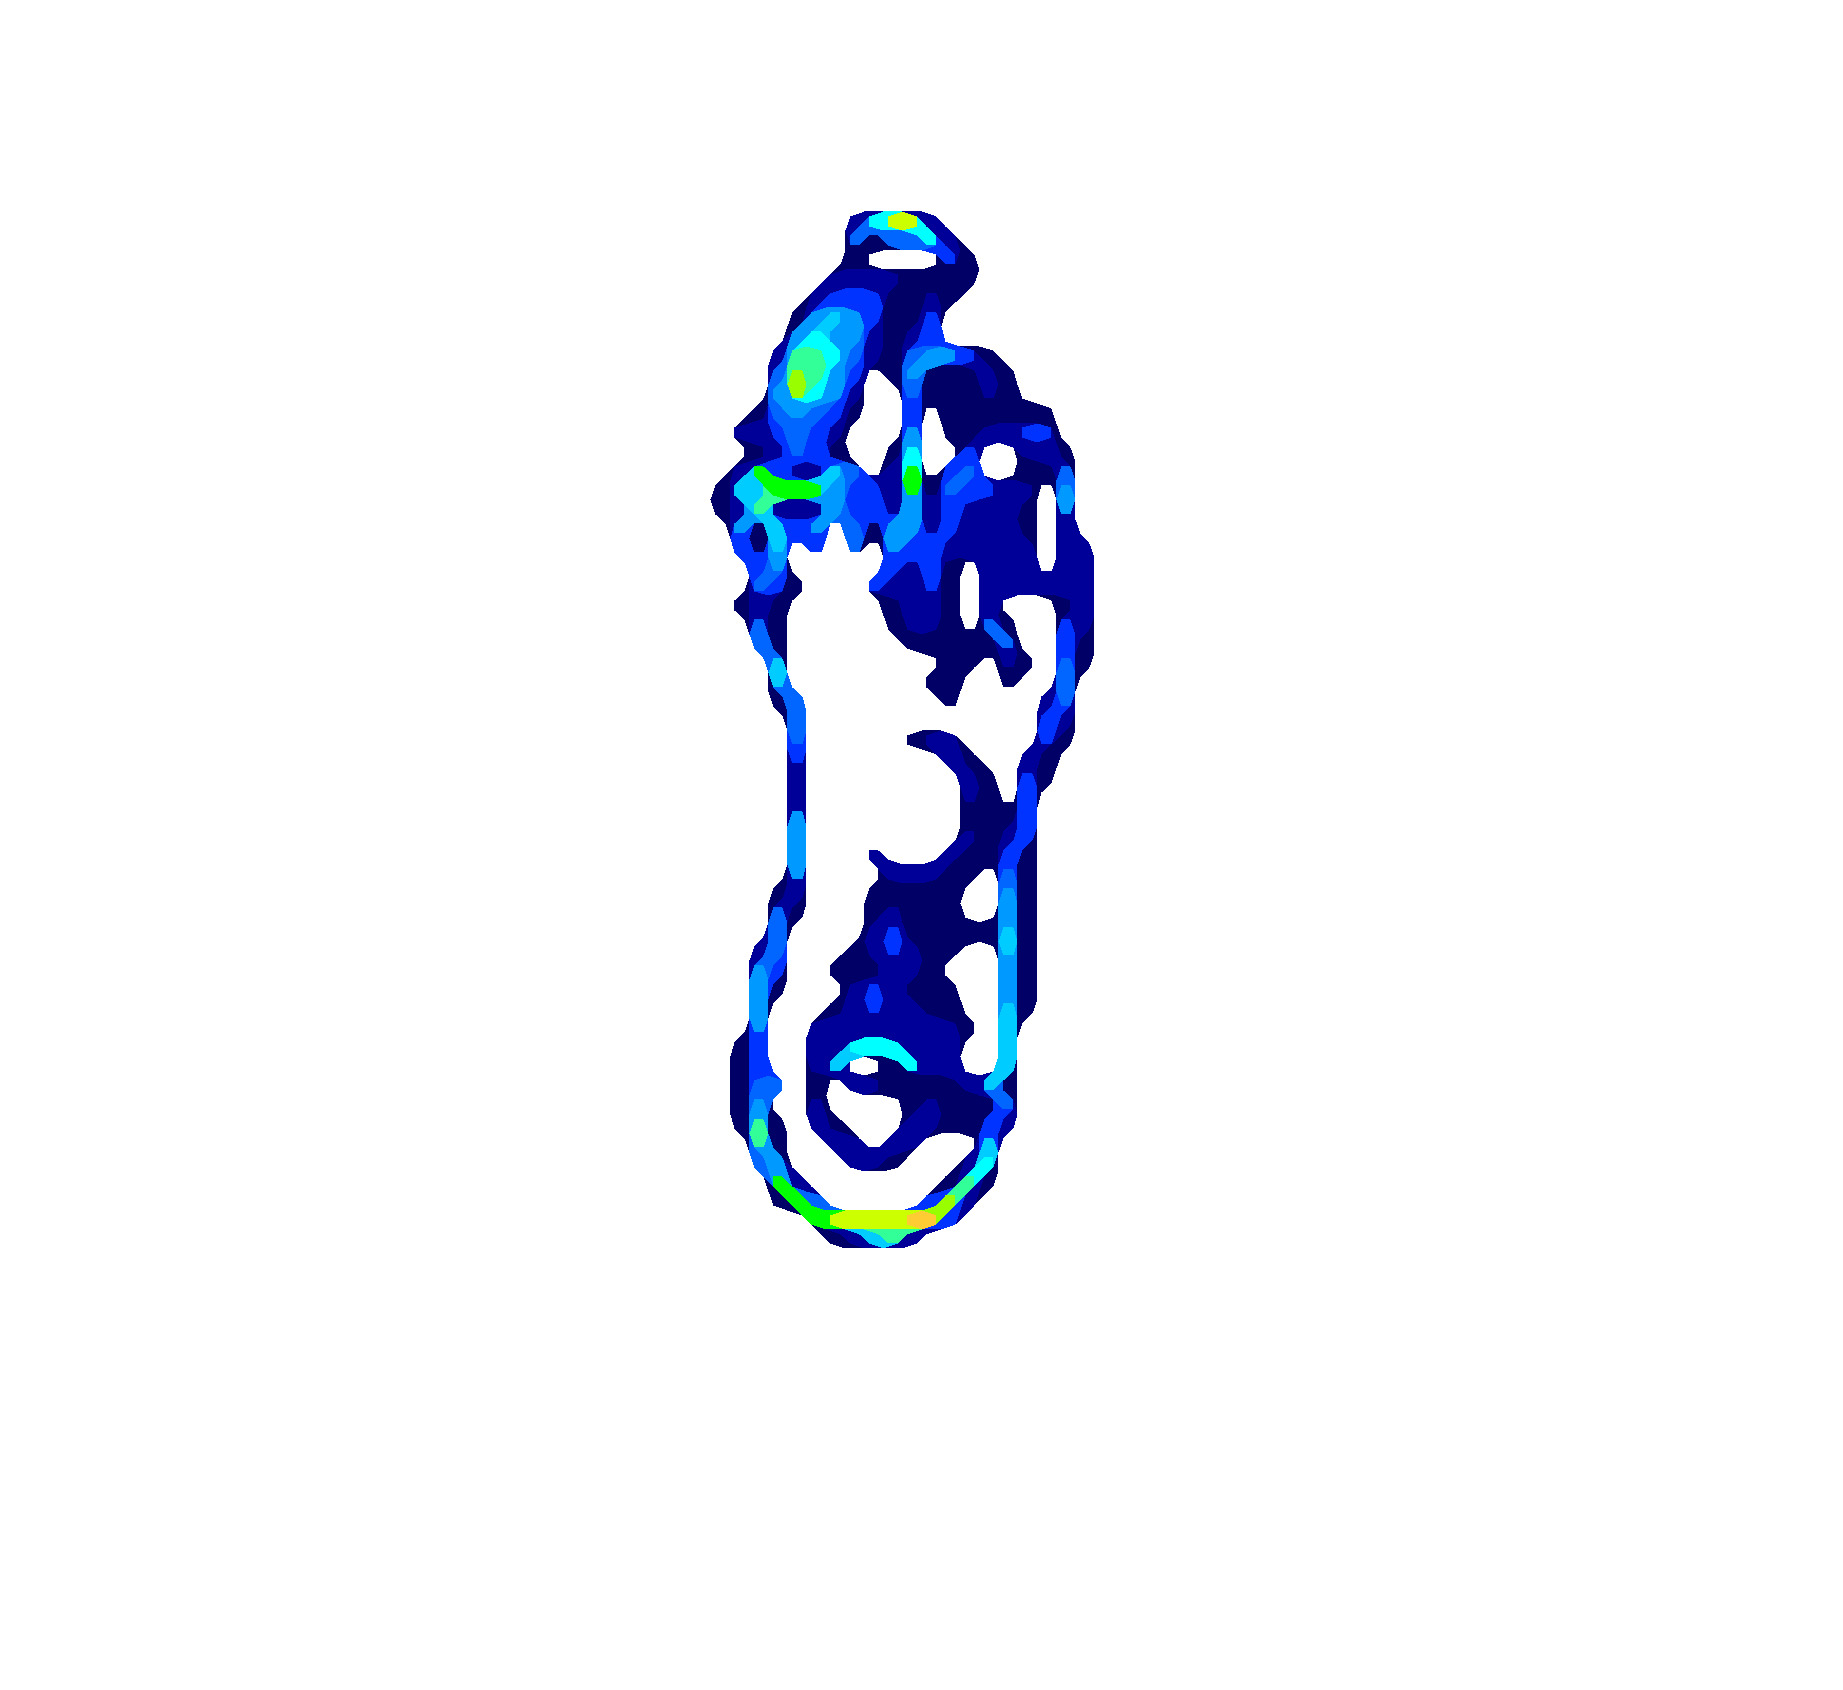
\includegraphics[width=8cm]{Mat_shoe}
\caption{Pressure map of a participants Adidas shoe taken on the Mat Pressure Scanner }
\label{Image 3}
\end{figure}

\newpage 

\subsubsection{High Resolution Photography}
 High resolution photographs were taken as both a reference and point of comparison for each pair of shoes. A Cannon camera was set up on a tripod and positioned above the shoe (Figure 4). Below the lens, the shoe was set into a plain, brown cardboard box that kept it stable.The shoe was then leveled in place using the technicians eye. Next to and on the same level as the shoe, a ruler, on a stand, was set up for scale. The tag from the bag was set next to it so that the date and shoe number could be seen in the final image (Figure 5). 
   
   The camera was hooked up to a laptop so that at no time did the research technician need to touch the camera itself. Two identical images were captured and saved as a jpg for each shoe. 

\begin{figure}[!htp]
\centering
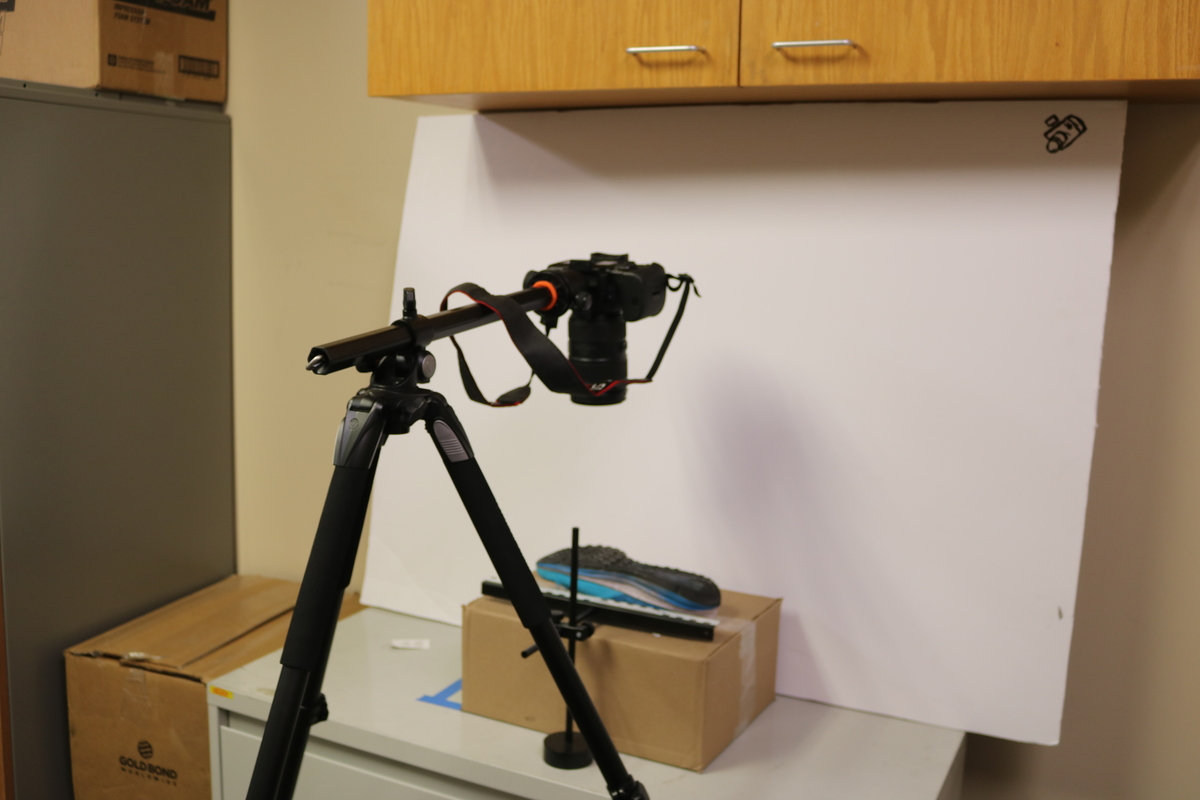
\includegraphics[width=8cm]{Original_Camera_Set}
\caption{The baseline camera set-up }
\label{Image 4}
\end{figure}

\begin{figure}[!htp]
\centering
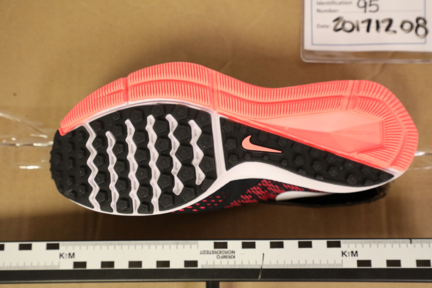
\includegraphics[width=8cm]{Baseline_Photo}
\caption{Sample of a baseline high resolution photograph}
\label{Image 5}
\end{figure}

\newpage

\subsubsection{2D Scanning}

 The Everspry 2D scanner was attached to a computer that had the specific software for the machine (Figure 6). The technician then put on the shoe to be scanned physically walked across the scanner. 
   
   For the purposes of this study, two walking methods were used when taking scans. For each shoe, the first two prints are detailed scans. The technician pointed their toe towards the ceiling and placed their heel on the scanner (Figure 7). Carefully, they then stepped down, placing all of their weight onto the shoe, and shifted their foot within. They then slowly peeled their foot up and stepped off of the scanner (Figure 8). The goal of this method was to get a clear scan with as much detail as possible. These four images, 2 per shoe, were then saved as STL files.
   
   The second method involved was a more realistic "walking print". The subject walked up to the scanner and then stepped onto the scanner. Immediately after, they step off as if walking down a road. These four images, 2 per shoe, were then saved as STL files.
   
   During baseline collection, the scanner was replaced with an identical model due to technical difficulties. The quality of the images and procedure remained unchanged (Figure 9). 

\begin{figure}[!htp]   
\centering
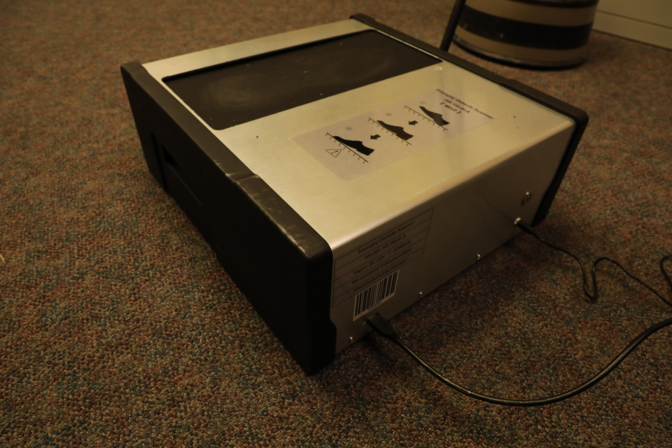
\includegraphics[width=8cm]{2D_Scanner}
\caption{2D Shoe sole scanner by Everspry}
\label{Image 6}
\end{figure}

\begin{figure}[!htp]   
\centering
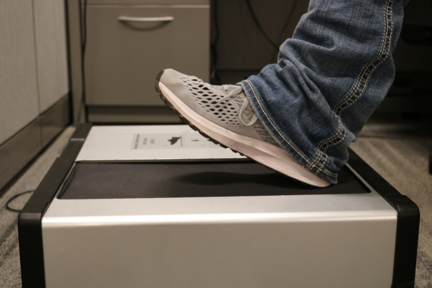
\includegraphics[width=8cm]{2D_Step_on}
\caption{Technician stepping onto the scanner}
\label{Image 7}
\end{figure}

\begin{figure}[!htp]   
\centering
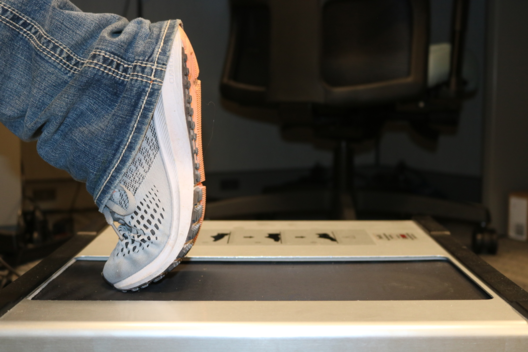
\includegraphics[width=8cm]{2D_Step_off}
\caption{Technician stepping off of the scanner}
\label{Image 8}
\end{figure}

\begin{figure}[!htp]
\centering
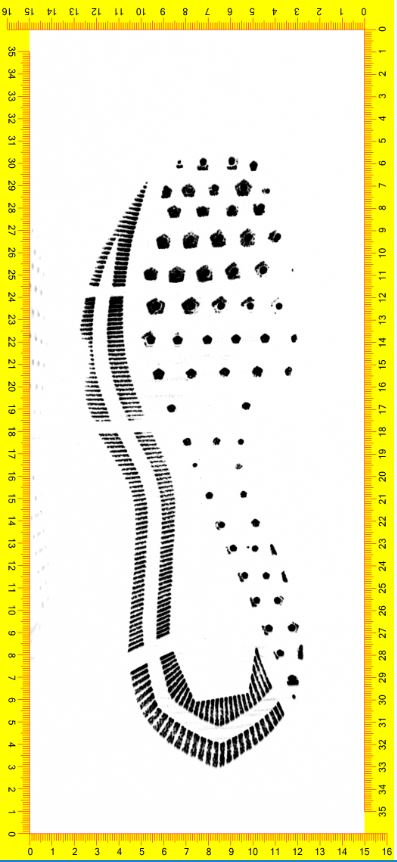
\includegraphics[width=4cm]{2D__Baseline_}
\caption{Scan of a Nike Winflo sole}
\label{Image 9}
\end{figure}


\newpage

\subsubsection{3D Scanning}

An EinScan-Pro+ hand held 3D scanner was used for this method (Figure 10). Once the software was installed,  technicians were able to take high quality three dimensional scans of shoe soles. 
   
   The shoe was placed on a stand which oriented the sole toward the technician. The scanner was then turned on and slowly moved back and forth across the shoe. The image could be seen coming together on the computer screen. green pixels covered the area being scanned and were then replaced by blue. After a rough image has been compiled, the technician adjusted the brightness of the scanner. This allowed the image to gain more detail. 
   
   The final image was a light blue digital rendering of the shoe sole (Figures 11-12)
   
\begin{figure}[!htp]
\centering
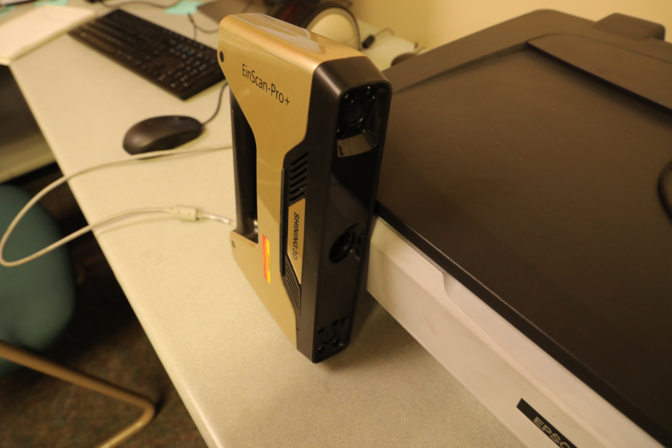
\includegraphics[width=8cm]{3D_Scanner}
\caption{Hand held 3D scanner: EinScan-Pro+}
\label{Image 10}
\end{figure}

\begin{figure}[!htp]
\centering
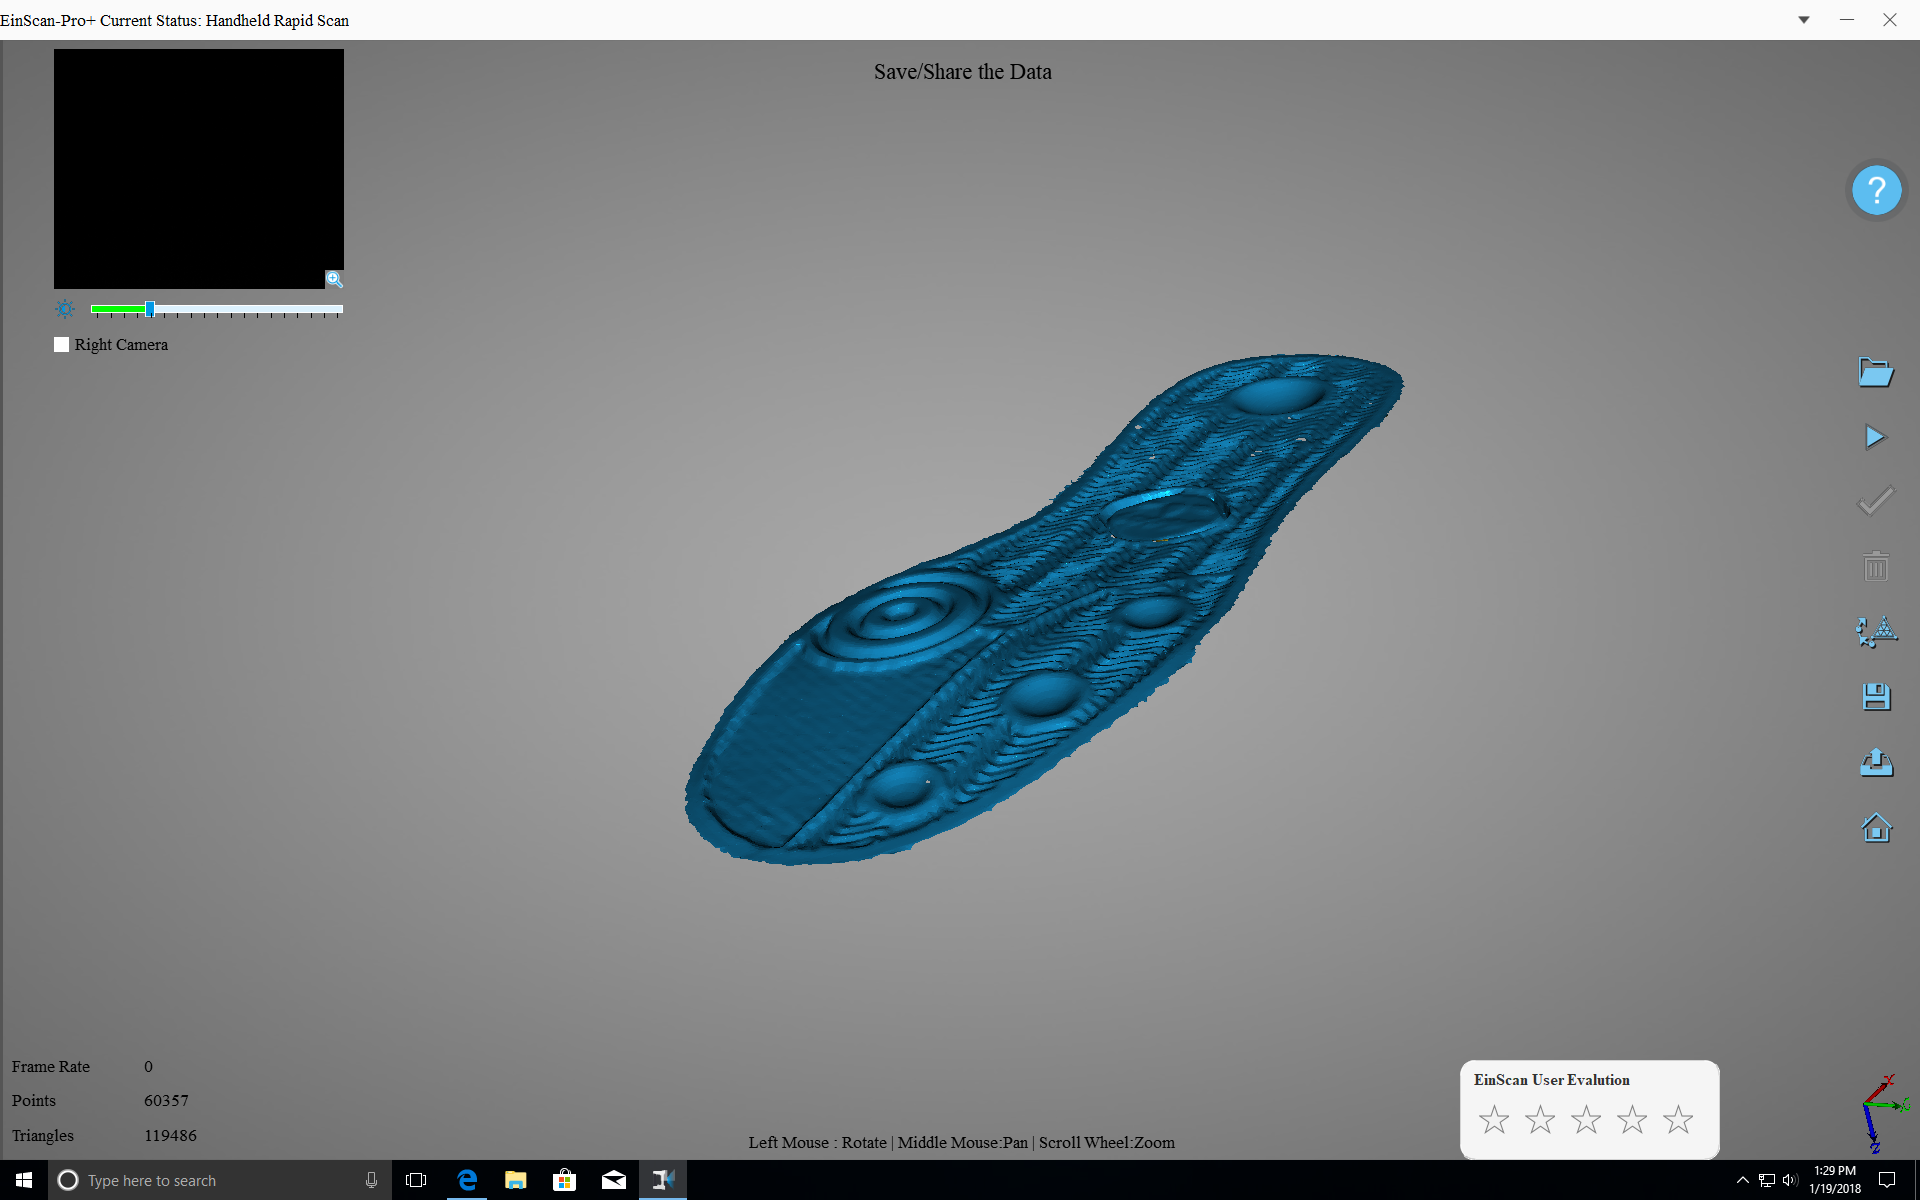
\includegraphics[width=8cm]{3D_Adidas}
\caption{On screen view when scanning an Adidas shoe sole}
\label{Image 11}
\end{figure}

\begin{figure}[!htp]
\centering
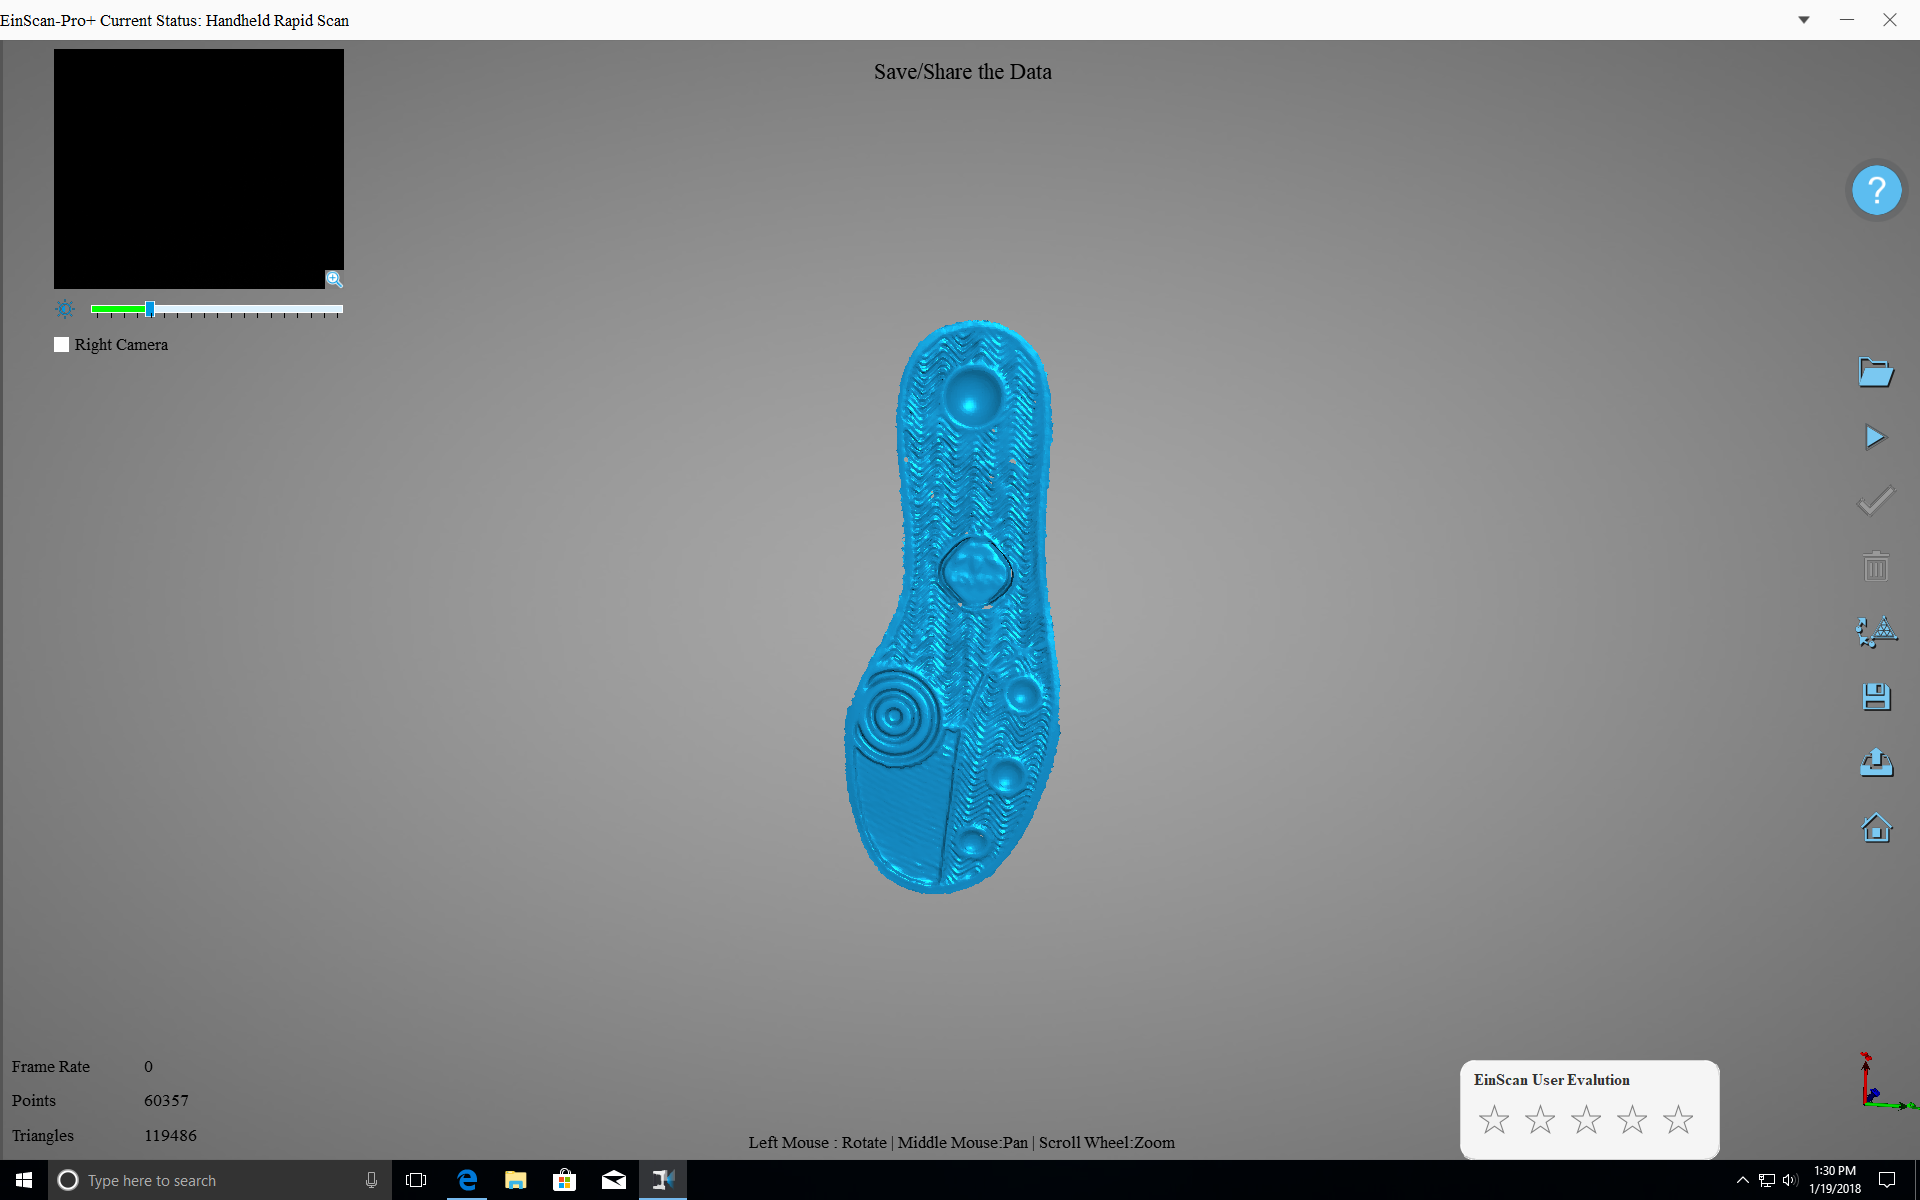
\includegraphics[width=8cm]{3D_Adidas_2}
\caption{On screen view when scanning an Adidas shoe sole}
\label{Image 12}
\end{figure}

\newpage

\subsubsection{Film Prints}

 This method involved using clear sticky films to take powder prints of the shoe soles. Two different types of film prints were taken, but the shoes were only brushed once per set. 
   
   The shoe soles were brushed with silver finger print powder, using a brush originally meant for finger printing. Canned, compressed air, held roughly 7 inches away, was then passed over the shoe soles in order to get rid of any excess powder. The shoe was then set aside and the other in the pair was powdered. 
   
   On the ground, newspaper was laid out and a chair was pulled up. While another technician put on one of the shoes, without touching the sole, the technician removed the clear film from its back. The film was placed on the newspaper in front of the subject, adhesive side facing up. Guiding their shoe down onto the film, the heel was placed on the film (Figure 13) with their toe pointing towards the ceiling. They then rolled their foot into a flat standing position and stepped up so that all of their weight was on the film. Weight was shifted in the shoe in order to capture all detail possible. 

   While the technician taking the print held the back corners (by the heel) of the film, carefully, the subject stepped off of the film, peeling the foot forward until only the tip of the toe was making contact with the adhesive. At this point, they stepped straight off, but did not place the powdered shoe on the ground. The back was then carefully replaced on the film and a label was placed on the back (Figure 14). 


   For the second print, a technician placed the clear portion, sticky side facing up, on the news paper near the subject. They then guided the subjects shoe down onto the paper. The subject placed their heel on the film with their toe pointing towards the ceiling. the foot was rolled into a flat standing position and and all weight was, again, placed on the film. They then lifted their foot, with the film attached, so that the sole was facing the technician. At this point, the technician manually pressed all portions of the film into the shoe, making sure to get all grooves and indents, if possible (Figure 15). After the film was thoroughly pressed in, the technician removed the film (Figure 16). The subject was then free to walk on the shoe. 
   
\begin{figure}[!htp]
\centering
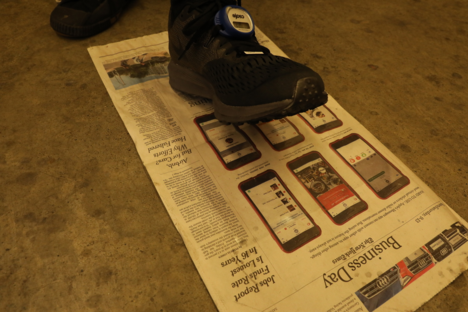
\includegraphics[width=8cm]{Film_Step}
\caption{Technician stepping onto a adhesive film}
\label{Image 13}
\end{figure}

\begin{figure}[!htp]
\centering
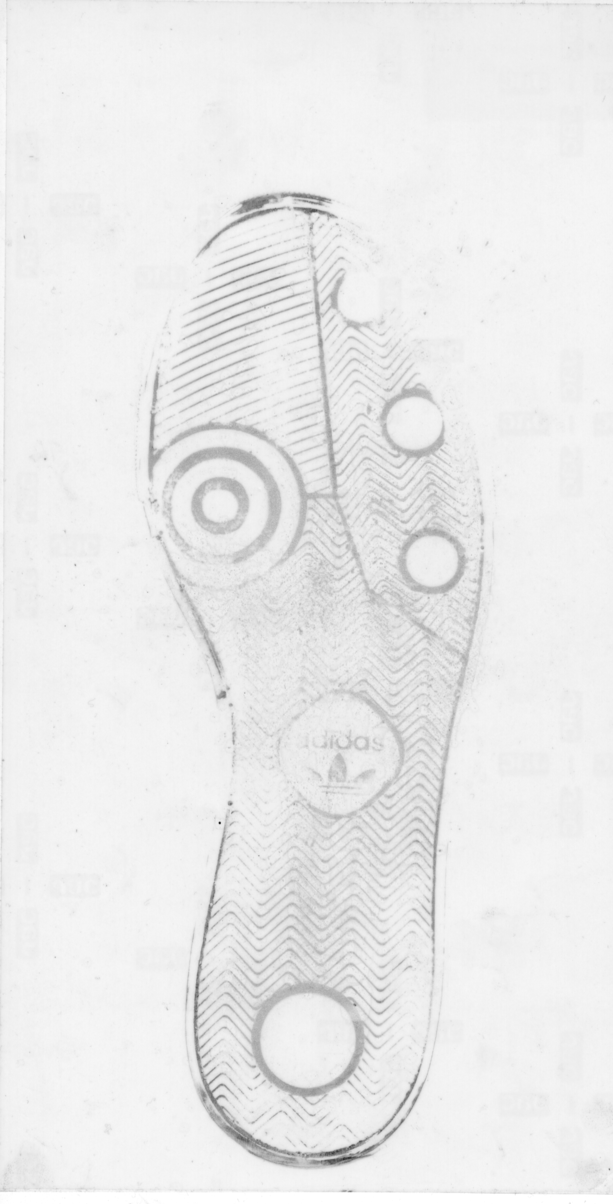
\includegraphics[width=4cm]{Film_1_Baseline}
\caption{Sample of a Baseline Film print 1}
\label{Image 14}
\end{figure}

\begin{figure}[!htp]
\centering
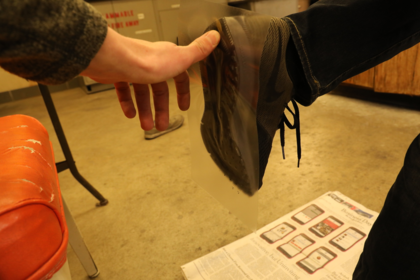
\includegraphics[width=8cm]{Press}
\caption{Technician pressing a film into a shoe sole}
\label{Image 15}
\end{figure}

\begin{figure}[!htp]
\centering
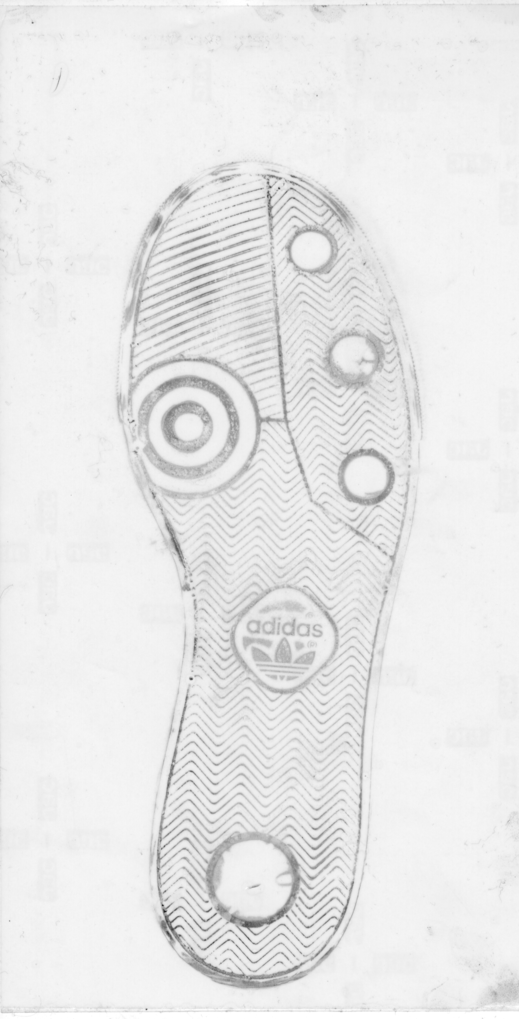
\includegraphics[width=4cm]{Film_2_Baseline}
\caption{Sample of a Baseline Film print 2}
\label{Image 16}
\end{figure}

\newpage

\subsubsection{Paper Prints}
 This method involved using 4 legal size pieces of printer paper, per shoe, to collect shoe prints that had been made with black fingerprint powder. Each shoe  generated 5 prints, but the shoes were only brushed once per set. This procedure flows into the Vinyl print procedure. 
   
     The shoe soles were brushed with black finger print powder using a brush originally meant for finger printing. Compressed air, held roughly 7 inches away, was then passed over the shoe soles in order to get rid of any excess dust. The shoe was then set aside and the other shoe in the pair was powdered. 
    
   A trail of 4 pieces of paper was laid end to end in front of another technician, who was sitting on a chair. At the very end of the trail, a piece of vinyl flooring was placed on the ground (Figure 17). The subject put on a powdered shoe without touching the sole. The technician not wearing the shoe then guided the subjects shoe down onto the paper. The subject placed their heel on the lower portion of the paper with their toe pointing towards the ceiling. They then rolled their foot into a flat standing position and stepped up so that all of their weight was concentrated on the shoe. The subject shifted their weight in the shoe in order to capture all detail possible (Figure 18). 

  At this point, the subject stepped straight off, but did not place the powdered shoe on the ground. On the second paper, they positioned the foot in the same way, but took a step as if walking normally. Again, they did not place the powdered shoe on the ground (Figure 19). 
  
  On the third paper, the subject stamped their foot straight down. At this point, they stepped straight off, but did not place the powdered shoe on the ground (Figure 20).
  
  On the fourth paper, the subject stepped and slightly twisted to smudge the print. They then stepped straight off, but did not place the powdered shoe on the ground (Figure 21).
  
  Lastly, the subject walked across the vinyl flooring that was laid at the end in the same way that they did for the second sheet of paper. 

   The completed prints were then labeled and laminated in order to protect the powder. The vinyl flooring pieces were labeled and set aside for later use. 
   
   These prints did not come out perfect. They were meant to simulate prints that would be found at a crime scene. 
   
\begin{figure}[!htp]
\centering
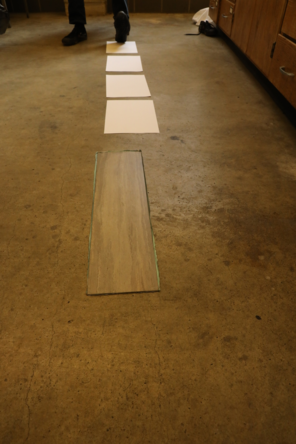
\includegraphics[width=5cm]{Path}
\caption{The path used for each, individual shoe.  }
\label{Image 17}
\end{figure}


\begin{figure}[!htp]
\centering
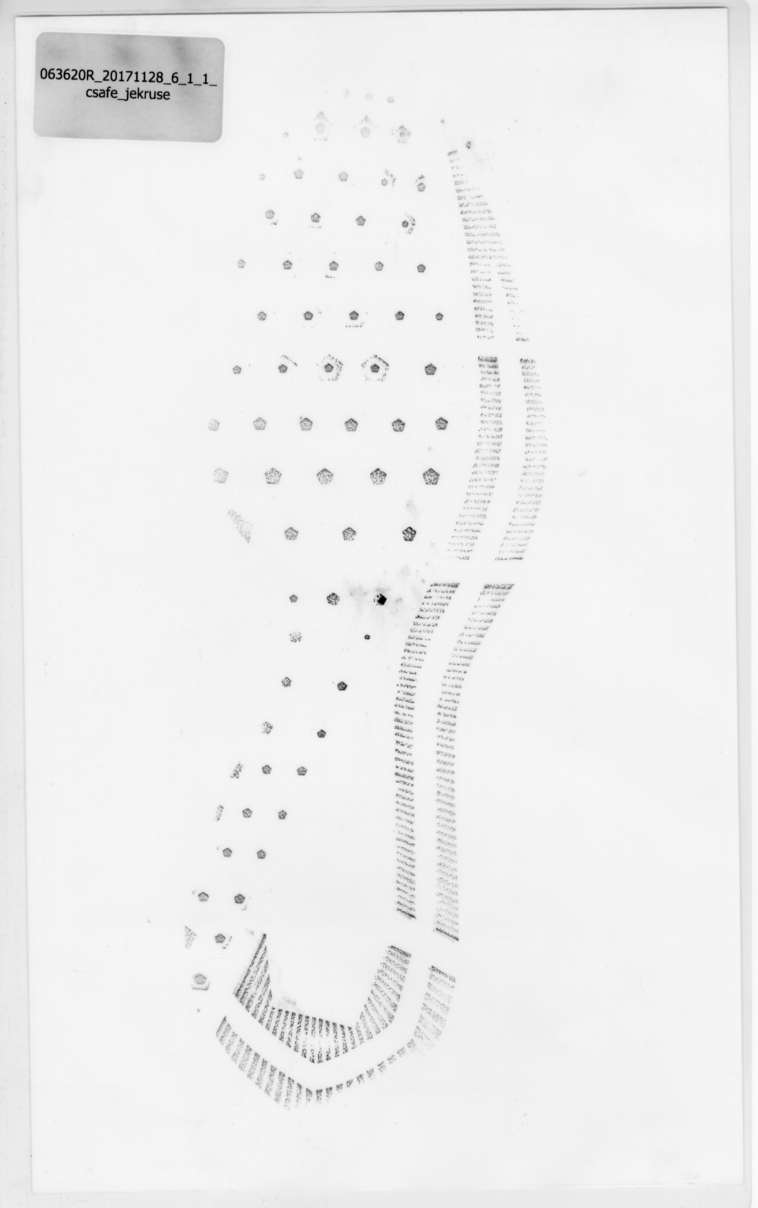
\includegraphics[width=4cm]{Baseline_Paper_1}
\caption{Sample of a Baseline paper print 1}
\label{Image 18}
\end{figure}

\begin{figure}[!htp]
\centering
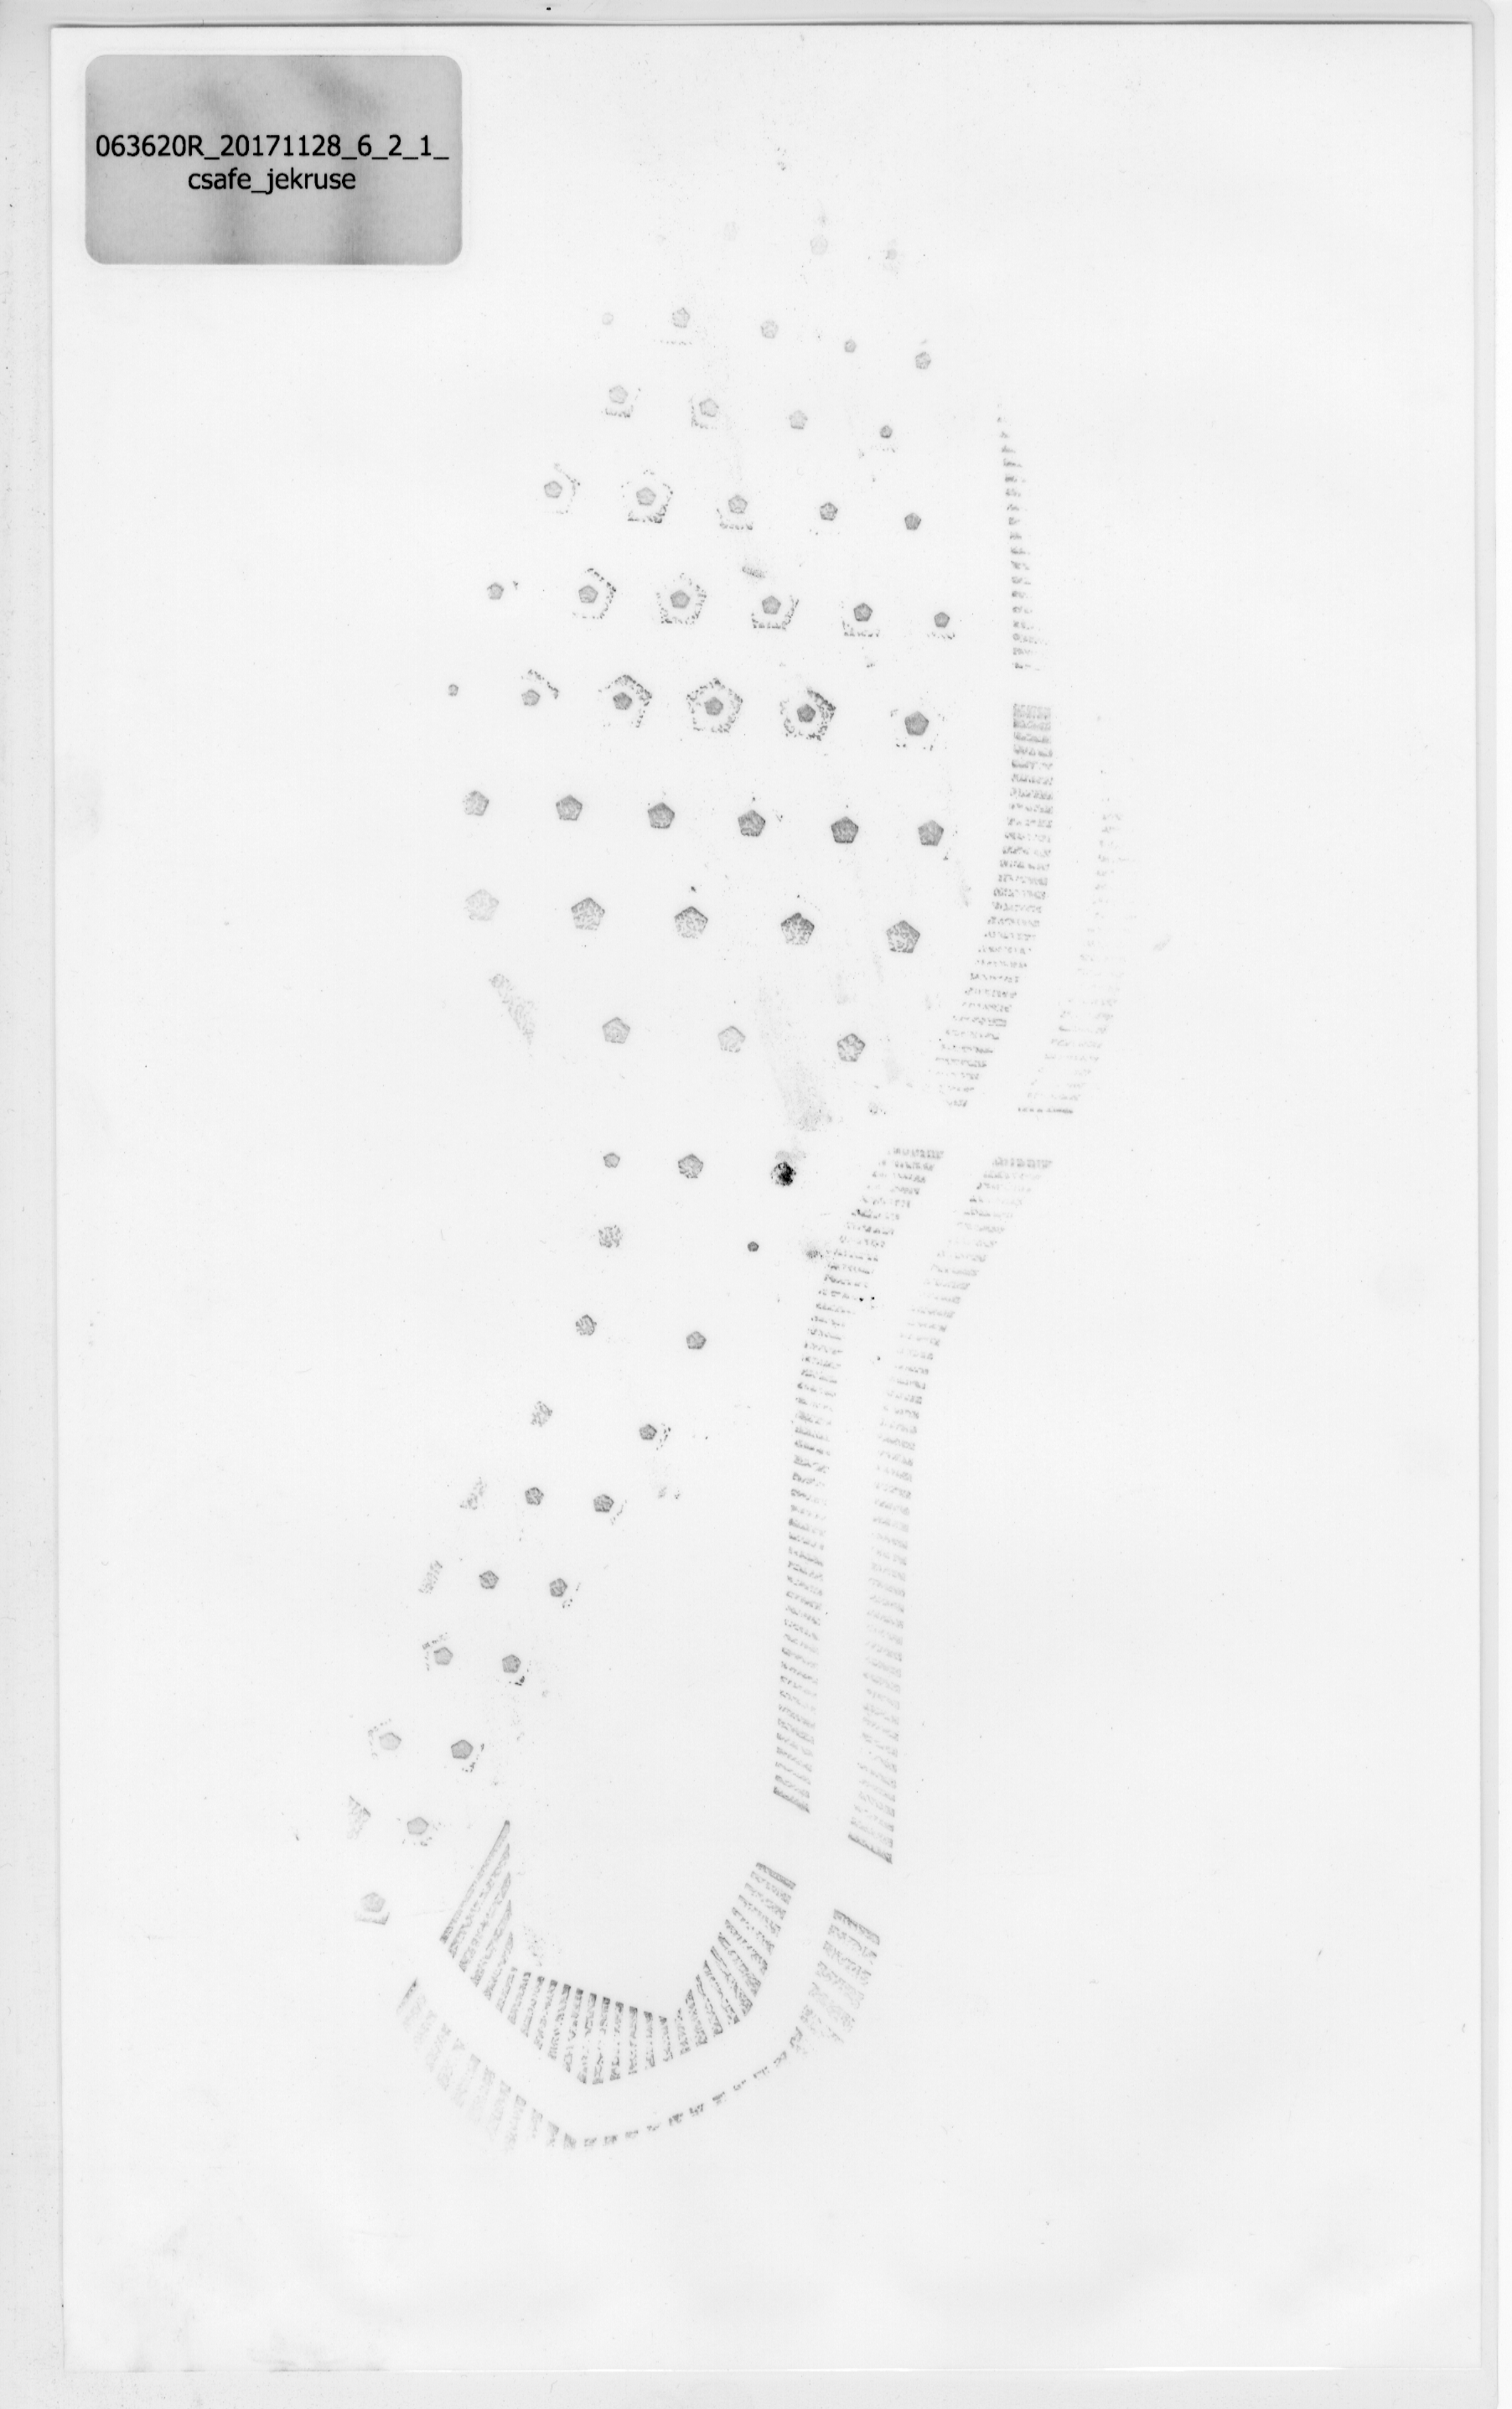
\includegraphics[width=4cm]{Baseline_Paper_2}
\caption{Sample of a Baseline paper print 2 }
\label{Image 19}
\end{figure}

\begin{figure}[!htp]
\centering
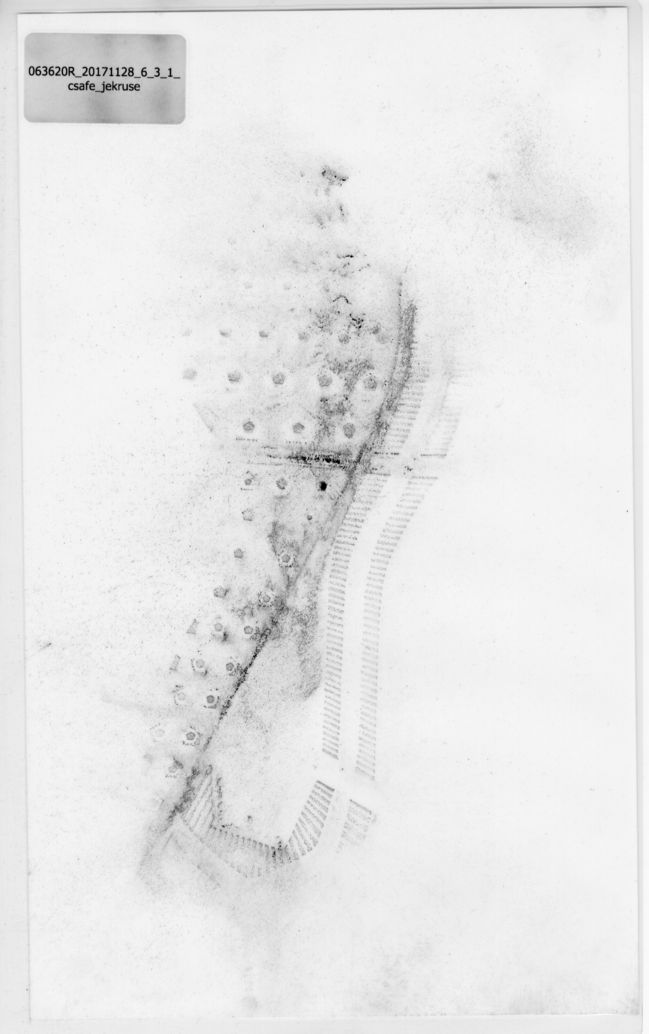
\includegraphics[width=4cm]{Baseline_Paper_3}
\caption{Sample of a Baseline paper print 3}
\label{Image 20}
\end{figure}

\begin{figure}[!htp]
\centering
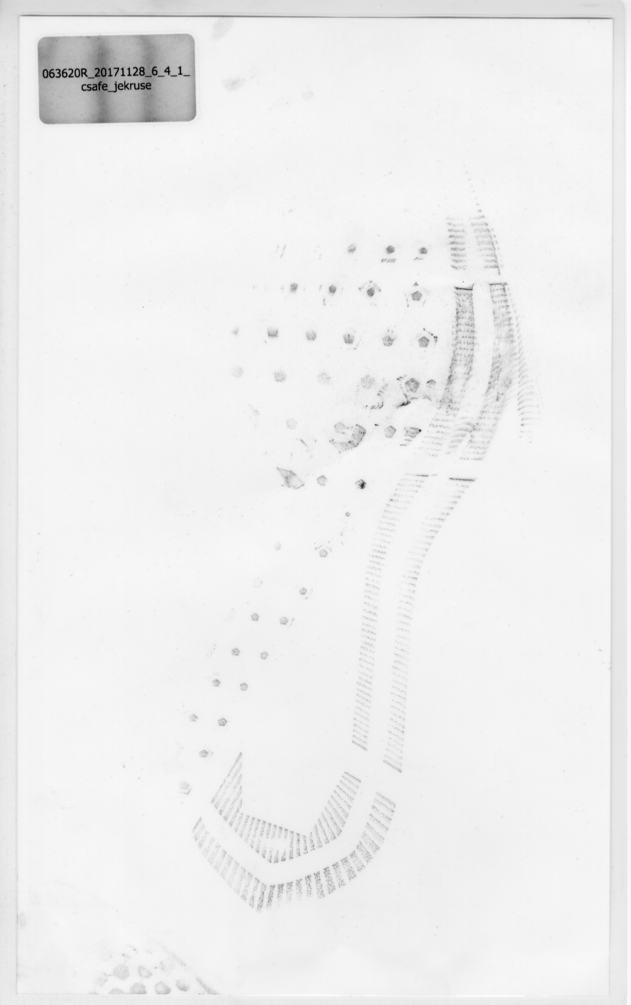
\includegraphics[width=4cm]{Baseline_Paper_4}
\caption{Sample of a Baseline paper print 4}
\label{Image 21}
\end{figure}

\newpage

\subsubsection{Vinyl Prints}

These pints were taken during the paper-print procedure.
   
   In the marked off area, the technician positioned the flooring and the lights on the pre-laid spike tape (Figure 22). A ruler was positioned next to the vinyl for scale. They then turned off the lights, computer monitors, and shut the door to make sure that light did not effect the photos.

   Standing overhead of the print and holding the camera, the technician took a photo straight down as if at a crime scene. The camera was zoomed in on the full print, even if the toe or heel was not completely visible. The lights were positioned as they are in the example images. They did not use the flash (Figure 23). Note: the label written in dry erase marker had to be visible in the photo.

   For the second photo, the tech altered the name written in marker to account for the second image, making sure not to damage the print. They took a second photo using the same procedure as before. 

   Once all photos had been taken, the vinyls were completely cleaned and allowed to dry. All files were saved as jpg. The images themselves were meant to simulate a print that was obtained from a household floor. 

Note: Not all images contain a scale placed at the side of the print. Images that did not have scale during the baseline collection are listed below.
\begin{itemize}

    \item - 1, 2, 3, 4, 5, 6, 7, 8, 9, 10, 11, 12, 13, 14, 15, 16, 17, 19, 20, 21, 23, 25, 28, 30, 123, 127, 129, 130, 131, 132, 133, 134, 136, 139, 144, 160
\end{itemize}

\begin{figure}[!htp]
\centering
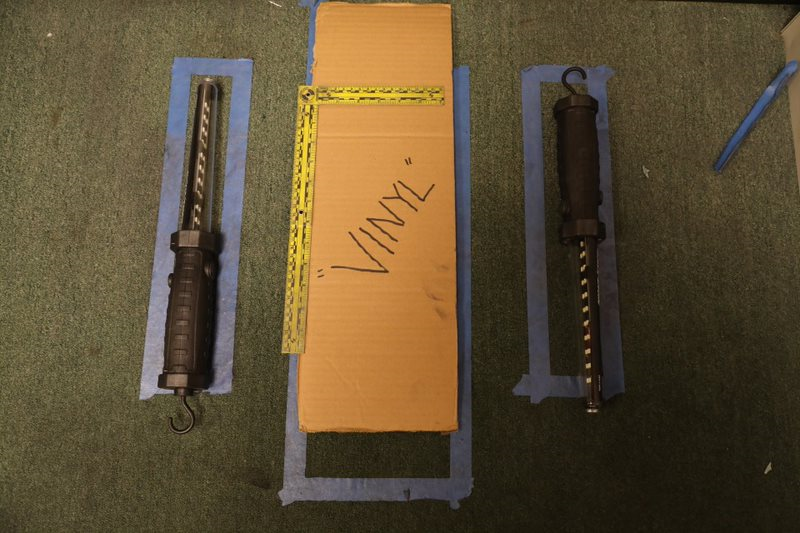
\includegraphics[width=8cm]{Baseline_Vinyl_set}
\caption{position of equipment when photographing vinyl crime scene replication prints}
\label{Image 22}
\end{figure}

\begin{figure}[!htp]
\centering
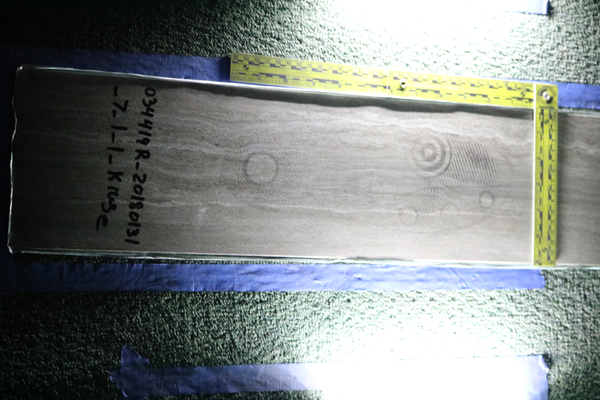
\includegraphics[width=8cm, angle=90]{Baseline_vinyl}
\caption{Vinyl crime scene replication prints being taken}
\label{Image 23}
\end{figure}

\newpage


\subsection{Collection 1}

\subsubsection{High Resolution Photography}
Starting with cohort 1, shoes were photographed, in most cases, before being powdered. 

Photos were taken using two different lighting systems (Figure 24). The first image was taken while being lit from the side by a shop light, with two individual light sources. The first light was lined up while the other was covered. Meanwhile, a night stick was facing the shoe. The second image was taken while being lit from the toe end of the shoe by the opposite shop light with the first one covered. The night stick was not facing the shoe. 

The camera shutter speed was altered as this point to allow for a longer exposure. 

All images were saved as TIFF files to allow for greater detail to be visible. 

\begin{figure}[!htp]
\centering
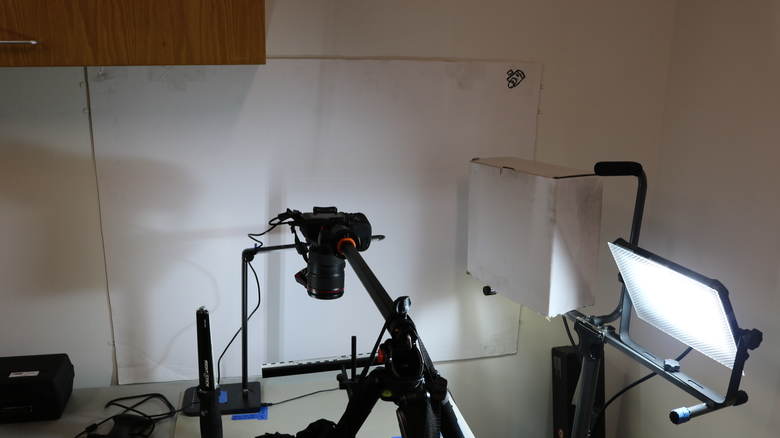
\includegraphics[width=8cm]{Camera_Lights}
\caption{A new lighting system was designed for high resolution photography}
\end{figure}

\subsubsection{2D Scanning}
There were no changes made to the 2D scanning procedure during this collection. 
\subsubsection{3D Scanning}
During this collection, shoes were scanned prior to being powdered. This created less interference with the lighting sources and resulted in a better scan. 
\subsubsection{Film Prints}
It was decided that a fume hood was needed for shoe powdering. For this reason, lab location moved and print quality improved. Fewer finger prints were present on films. 

During this collection, a quarter inch of foam was placed under the news paper. The films were then powdered and placed the same way. This procedure change yielded more detail in the first print. 

Due to the possibility of double prints, the procedure for the second print changed. This new procedure yielded a clearer image, but the toe of each shoe was lost (Figure 25). This change went into effect between cohort 1 and cohort 2 collection. The new procedure is given below. 

 "For the second print, technicians placed the film, adhesive side facing up, on the news paper, with the foam underneath, near the subject. A technician then guided the subjects shoe down onto the paper. The subject placed their heel on the film with their toe pointing towards the ceiling. They then rolled their foot into a flat standing position and stepped up so that all of their weight was on the film. They then lifted their foot straight up, making sure not to shift the shoe on the film. The technician then carefully pulled the film off of the shoe, making sure to only grab the film by the corner. The subject was then free to walk on the shoe." 
 
\begin{figure}[!htp]
\centering
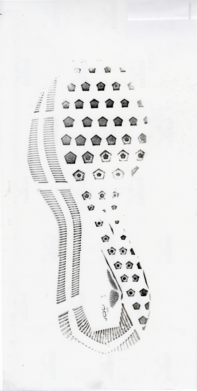
\includegraphics[width=4cm]{New_Film}
\caption{Sample of a revised film print 2}
\label{Image 25}
\end{figure}

\newpage

\subsubsection{Paper Prints}
Near the end of collection one, it was decided that a fume hood was needed for shoe powdering.For this reason, lab location moved and print quality improved. Fewer finger prints were present on papers. 
\subsubsection{Vinyl Prints}
There were no changes made to the vinyl prints procedure during this collection.

\newpage


\subsection{Collection 2}

\subsubsection{High Resolution Photography}
At the suggestion of an expert shoe print examiner, shoes were placed in a box that had been covered in grid paper. This began during cohort two.

A green rectangle started getting placed around the shoes between cohort three and cohort four to assist with later analysis (Figure 26). 

Technicians began using a bubble level during analysis to make sure that the shoe was as level as possible. 

The stand ruler that had been used for scale was replaced by a flat "L" ruler during the collection of cohort 3. This ruler was placed on the box stand itself (Figure 27). 

The lighting difference between image 1 and image two altered. The night stick rotation was removed and instead it remained facing the shoe for both images.

\begin{figure}[!htp]
\centering
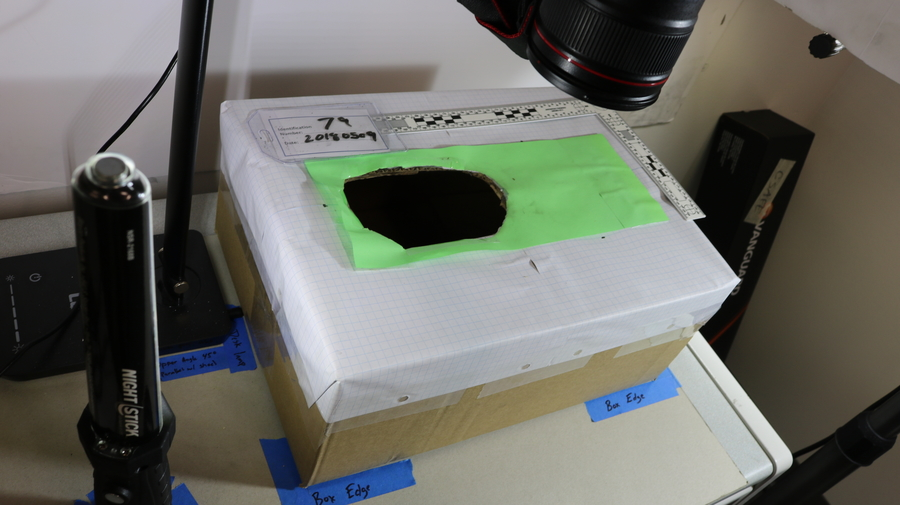
\includegraphics[width=8cm]{New_Box}
\caption{Updated box for high resolution photography}
\label{Image 26}
\end{figure}

\begin{figure}[!htp]
\centering
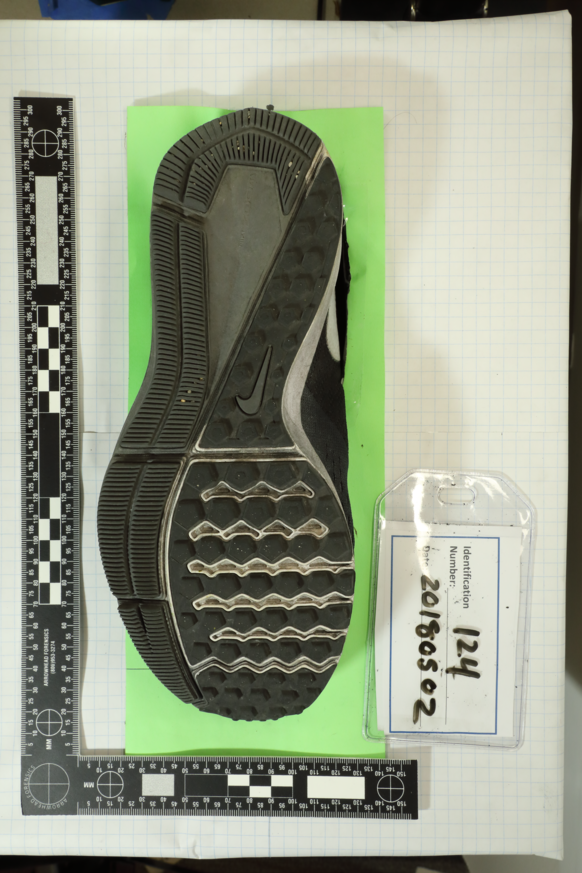
\includegraphics[width=5cm]{New_Photo}
\caption{Sample of a revised photo }
\label{Image 27}
\end{figure}

\newpage

\subsubsection{2D Scanning}
There were no changes made to the 2D scanning procedure during this collection.

\subsubsection{3D Scanning}
There were no changes made to the 3D scanning procedure during this collection.

\subsubsection{Film Prints}
An air compressor was put into use during this collection to eliminate the need for cans of compressed air. The same procedure was used.

\subsubsection{Paper Prints}
An air compressor was put into use during this collection to eliminate the need for cans of compressed air. The same procedure was used.
\subsubsection{Vinyl Prints}
   During the collection of cohort 1, the yellow, collapsible ruler was exchanged for a white "L" ruler. This would remain the norm for the majority of the remaining photos. A yellow ruler was used again near the end of collection 3. 

   During the collection of cohort 1, the camera began getting put on a tripod instead of being held by the technician. The same procedure was used and the button was still manually pressed by the technician. 
   
   During the collection of cohort 2, two blank pieces of vinyl flooring were placed on either side of the print. The paper along the edges of the individual pieces were slowly  removed from this point on (Figure 28). 
   
\begin{figure}[!htp]
\centering
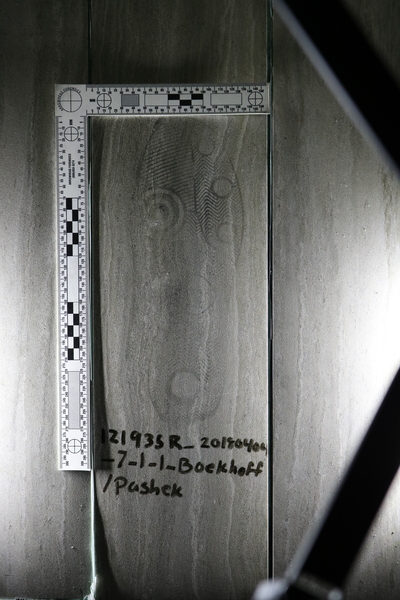
\includegraphics[width=5cm]{New_Vinyl}
\caption{Sample of a revised vinyl photo}
\label{Image 28}
\end{figure}

\newpage


\subsection{Collection 3}

\subsubsection{High Resolution Photography}
At the suggestion of experts in shoe print examination, both the stand ruler and the flat "L" ruler were used. This was to give a scale at the shoes hight and still keep a consistent scale across images. This change was put into place for only the last few images (Figure 29). 

\begin{figure}[!htp]
\centering
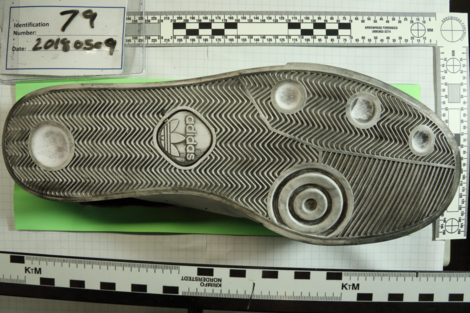
\includegraphics[width=7cm]{New_photo__2_}
\caption{Sample of a revised high resolution photo}
\label{Image 29}
\end{figure}

\subsubsection{3D Scanning}
There were no changes made to the 3D scanning procedure during this collection. 
\subsubsection{2D Scanning}
Due to residue build-up from past cleanings, the cleaning procedure was changed to eliminate the possibility of any cloudiness or artifacts in the 2D images. The was done after data collection on cohort 2 had concluded. 
\subsubsection{Film Prints}
There were no changes made to the paper print procedure during this collection. 
\subsubsection{Paper Prints}
There were no changes made to the paper print procedure during this collection. 
\subsubsection{Vinyl Prints}
There were no changes made to the vinyl prints procedure during this collection.

\newpage

\subsection{Files Saved Incorrectly}

   During the course of the study, some files, models, and/or images were incorrectly saved. Below, files have been listed that were saved in a format different from what was required/listed. 
   
\begin{itemize}
\item Cohort 2, Check in 1, 3D SCan, 040683R-20180205-3-1-1-bpbryson.asc
\item Cohort 5, Check in 2, 3D SCan, 144363L-20180404-3-1-1-jekruse.asc
\item Cohort 5, Check in 1, 2D SCan, 144088R-20180221-2-2-1-dtmartin.jpg -> Changed to TIFF
\item Cohort 5, Check in 1, 2D SCan, 130829R-20180221-2-2-1-hanrahan.bmp -> Changed to TIFF
\end{itemize}
   

\end{document}